\documentclass{article}

\usepackage{ipprocess}
%\usepackage{lmodern}
\usepackage{longtable}
\usepackage[latin1]{inputenc} 
\usepackage[T1]{fontenc}
\pagestyle{fancy}
\usepackage{libertine}

%\usepackage[author={Jo�o Carlos Nunes Bittencourt}]{pdfcomment}

\sloppy

\title{32-bit uDLX Core Processor}

\graphicspath{{./pictures/}} % Diret�rio padr�o de figuras.
\makeindex
\begin{document}
  \capa{1.0}{abril}{2014}{32-bit uDLX Core Processor}{Architecture Specification}{Universidade Federal da Bahia}
  \newpage

%%%%%%%%%%%%%%%%%%%%%%%%%%%%%%%%%%%%%%%%%%%%%%%%%%
%% GNU LGPL Licence
%%%%%%%%%%%%%%%%%%%%%%%%%%%%%%%%%%%%%%%%%%%%%%%%%%

  
\begin{center}
\begin{Large}\textbf{GNU LGPL License}                          \end{Large}
\end{center}
\vspace{2cm}
\fbox{
  \parbox{.7\textwidth}{
    \vspace{0,5cm}
    \begin{scriptsize}
    This file is part of uDLX (micro-DeLuX) soft IP-core.\\

    uDLX is free soft IP-core: you can redistribute it and/or modify
    it under the terms of the GNU General Public License as published by
    the Free Software Foundation, either version 3 of the License, or
    (at your option) any later version.\\

    uDLX soft core is distributed in the hope that it will be useful,
    but WITHOUT ANY WARRANTY; without even the implied warranty of
    MERCHANTABILITY or FITNESS FOR A PARTICULAR PURPOSE. See the
    GNU General Public License for more details.

    You should have received a copy of the GNU General Public License
    along with uDLX. If not, see <http://www.gnu.org/licenses/>.
    \end{scriptsize}
    \vspace{0,5cm}
  }
}

\newpage

%%%%%%%%%%%%%%%%%%%%%%%%%%%%%%%%%%%%%%%%%%%%%%%%%%
%% Hist�rico de Revis�es
%%%%%%%%%%%%%%%%%%%%%%%%%%%%%%%%%%%%%%%%%%%%%%%%%%
  \section*{\center Hist�rico de Revis�es}
  \vspace*{1cm}
  \begin{table}[ht] % aqui come�a o ambiente tabela
  \centering
  \begin{tabular}[pos]{|m{2cm} | m{7.2cm} | m{3.8cm}|} 
  \hline % este comando coloca uma linha na tabela
  \cellcolor[gray]{0.9}
  \textbf{Date} & \cellcolor[gray]{0.9}\textbf{Description} & \cellcolor[gray]{0.9}\textbf{Author(s)}\\ \hline
  \hline
  \small 04/27/2014 & \small Conception & \small Jo�o Carlos Bittencourt \\ \hline
  \small 04/30/2014 & \small Instruction layout description & \small Jo�o Carlos Bittencourt \\ \hline
  \small 05/09/2014 & 
  \begin{small}
    \begin{itemize}
      \item Text revision;
      \item Update diagrams and instruction layout;
      \item Update instruction fetch I/O definitions;
      \item Missing pictures inclusion;
      \item Include memory access and write back pin/port definitions;
    \end{itemize}
  \end{small} & \small Jo�o Carlos Bittencourt \\ \hline
  \small 04/13/2014 & \small Missing pictures & \small Jo�o Carlos Bittencourt \\ \hline
  \small 04/15/2014 & \small   \begin{small}
    \begin{itemize}
      \item Fix instruction fetch pin definitions;
      \item Include instruction fetch datapath;
      \item Include pipeline registers definitions;
      \item Fix memory access stage pin/port definitions;
      \item Include write back data path;
    \end{itemize}
  \end{small} & \small Jo�o Carlos Bittencourt \\ \hline
  \small 04/15/2014 & \small Add execute block diagram & \small Igo Amauri Luz \\ \hline
  \small 04/16/2014 & \small   \begin{small}
    \begin{itemize}
      \item Add branch prediction signal to ID and IF blocks and pin definitions;
      \item Add table for pin definitions in Execute stage
      \item Add branch prediction signal in pipeline registers definitions;
    \end{itemize}
  \end{small} & \small Jo�o Carlos Bittencourt \\ \hline  
  \end{tabular}
  \label{tab:revisoes}
  \end{table}

  \newpage
  
  \tableofcontents
  \newpage

%%%%%%%%%%%%%%%%%%%%%%%%%%%%%%%%%%%%%%%%%%%%%%%%%%
%% Concent
%%%%%%%%%%%%%%%%%%%%%%%%%%%%%%%%%%%%%%%%%%%%%%%%%%
  \section{Introduction}
  \subsection{Purpose}
  The main purpose of this document is to define specifications of a uDLX implementation and to provide a full overview of the design. This specifications defines all implementation parameters that composes the general uDLX requirements and specification. This definitions include processor operation modes, instruction set (ISA) and internal registers characteristics. This document also include detailed information of pipeline stages architecture, buses and other supplemental units.
  
  \subsection{Document Outline Description}
  This document is outlined as follow:
	
	\begin{itemize}
	  \item Section \color{black}{\ref{sec:architecture_overview}}: This section presents the core processor block diagram, Pin/Port definitions and global parameters and configuration directives.
	  \item Section \color{black}{\ref{sec:instruction_layout}}: This section presents the $\mu$DLX instruction layout and specifications. 
    \item Section \color{black}{\ref{sec:architecture_description}}: This section presents a description of each pipeline stage block, including pin definitions, signals and internal datapath.
	\end{itemize}
		
  \subsection{Acronyms and Abbreviations}
  Along this and other documents part of this project, it will be recurrent the usage of some acronyms and abbreviations. In order to keep track of this elements the Table \ref{tab:definitions} presents a set of abbreviations used and its corresponding meaning.
  
  \FloatBarrier
  \begin{table}[H] % aqui come�a o ambiente tabela
    \begin{center}
      \caption{Acronym and descriptions of elements in this document.}
      \label{tab:definitions}

      \begin{tabular}[pos]{|m{2cm} | m{9cm}|} 
	\hline % este comando coloca uma linha na tabela
	\cellcolor[gray]{0.9}\textbf{Acronym} & \cellcolor[gray]{0.9}\textbf{Description} \\ \hline
	RISC & Reduced Instruction Set Computer \\ \hline
	GPR & General Purpose Registers \\ \hline
	FPGA & Field Gate Programmable Array \\ \hline
	GPPU & General Purpose Processing Unit \\ \hline
	SDRAM & Synchronous Dynamic Random Access Memory\\ \hline
	HDL & Hardware Description Language \\ \hline
	RAW & Read After Write \\ \hline
	CPU & Central Processing Unit \\ \hline
	ISA & Instruction Set Architecture \\ \hline
	ALU & Arithmetic and Logic Unit \\ \hline
	PC  & Program Counter \\ \hline
	RFlags & Flags Register \\ \hline
	Const  & Constant \\ \hline
  BPM    & Branch Prediction Buffer \\ \hline
      \end{tabular}
    \end{center}
  \end{table}
  
  \newpage
  \section{Architecture Overview}
  \label{sec:architecture_overview}
  
  \subsection{Block Diagram}
  \begin{figure}[H]
    \centering
    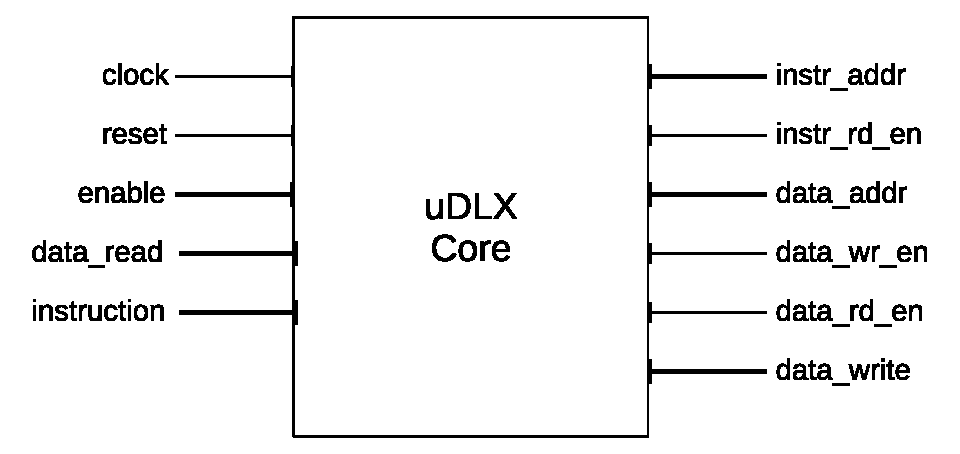
\includegraphics[width=.8\linewidth]{pictures/udlx_block.eps}
  \label{fig:datapath}
  \end{figure}
 
 
  \subsection{Pin/Port Definitions}
  \FloatBarrier
  \begin{table}[H]
    \begin{center}
      \begin{tabular}[pos]{| l | c | c | m{7cm} |} \hline 	
      \multicolumn{1}{|c|}{\cellcolor[gray]{0.9}\textbf{Name}} & 
      \multicolumn{1}{c|}{\cellcolor[gray]{0.9}\textbf{Length}} & 
      \multicolumn{1}{c|}{\cellcolor[gray]{0.9}\textbf{Direction}} &
      \multicolumn{1}{c|}{\cellcolor[gray]{0.9}\textbf{Description}} \\ \hline
	 clock 		& 1 	& input 	& CPU core clock  	\\ \hline
	 reset 		& 1	& input		& CPU core reset  	\\ \hline
	 sram\_data\_io 	& 16	& in/out 	& SRAM data \\ \hline
	 sdram\_data\_io 	& 32	& in/out 	& SDRAM data \\ \hline
	 sram\_addr 	& 20	& input 	& SRAM address \\ \hline
	 sram\_we\_n 	& 1	& output 	& SRAM write enable  \\ \hline
	 sram\_oe\_n 	& 1	& output 	& SRAM output enable  \\ \hline
	 sdram\_addr 	& 13	& in/out	& SDRAM address \\ \hline
	 sdram\_we 	& 1	& output 	& SDRAM write enable  \\ \hline
	 sdram\_oe 	& 1	& output 	& SDRAM output enable  \\ \hline
      \end{tabular}
    \end{center}
  \end{table}  
   
  \subsection{Parameters and Configurations}

 \FloatBarrier
  \begin{table}[H]
    \begin{center}
      \begin{tabular}[pos]{| l | l | m{8cm} |} \hline 	
      \multicolumn{1}{|c|}{\cellcolor[gray]{0.9}\textbf{Name}} & 
      \multicolumn{1}{c|}{\cellcolor[gray]{0.9}\textbf{Value}} & 
      \multicolumn{1}{c|}{\cellcolor[gray]{0.9}\textbf{Description}} \\ \hline
	  & &  	\\ \hline
      \end{tabular}
    \end{center}
  \end{table} 
    
  \newpage
  \section{Instructions Layout}
  \label{sec:instruction_layout}

  \subsection{ALU}
  \begin{figure}[H]
    \centering
    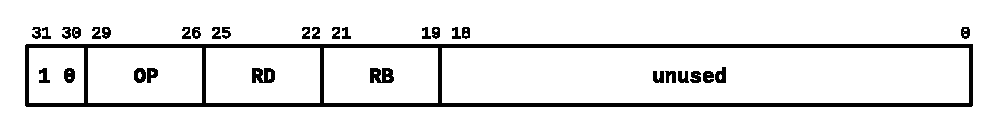
\includegraphics[width=\linewidth]{pictures/alu_instruction.eps}
  \end{figure} 
  
  \FloatBarrier
  \begin{table}[H]
    \begin{center}
      \begin{tabular}[pos]{| c | l | l | l |} \hline 	
      \multicolumn{1}{|c|}{\cellcolor[gray]{0.9}\textbf{OP}} & 
      \multicolumn{1}{c|}{\cellcolor[gray]{0.9}\textbf{Opperation}} & 
      \multicolumn{1}{c|}{\cellcolor[gray]{0.9}\textbf{Mnemonic}} &
      \multicolumn{1}{c|}{\cellcolor[gray]{0.9}\textbf{Flags Update}} \\ \hline
	 0000 & $R_D = R_D + R_F$ 	& add d, f 	& all	 \\ \hline
	 0001 & $R_D = R_D - R_F$ 	& sub d, f 	& all 	\\ \hline
	 0010 & $R_D = R_D * R_F$ 	& mul d, f 	& all	\\ \hline
	 0011 & $R_D = R_D / R_F$ 	& div d, f 	& all	\\ \hline
	 0100 & $R_D = R_D~and~R_F$ 	& and d, f 	& above, equal, error \\ \hline
	 0101 & $R_D = R_D~or~R_F$ 	& or d, f 	& above, equal, error \\ \hline
	 0110 & $R_flags = R_D~cmp~R_F$ 	& cmp d, f 	& above, equal, error \\ \hline
	 0111 & $R_D =~not~R_D $		& not d 	& above, equal, error \\ \hline
      \end{tabular}
    \end{center}
  \end{table} 
  
  \subsection{Immediate}
  
  \textbf{Type I}
  \begin{figure}[H]
    \centering
    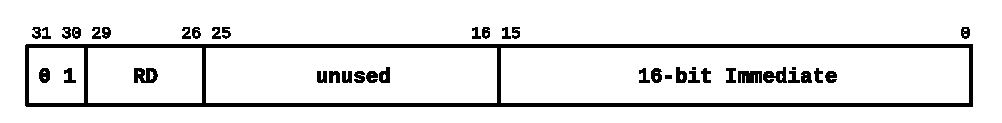
\includegraphics[width=\linewidth]{pictures/immediate_type_1.eps}
  \end{figure}  
  
  \hspace{-36px}\textbf{Type II}  
  \begin{figure}[H]
    \centering
    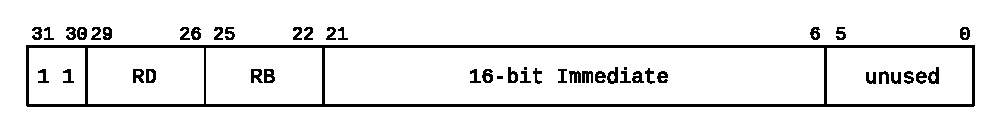
\includegraphics[width=\linewidth]{pictures/immediate_type_2.eps}
  \end{figure}  
  
  \FloatBarrier
  \begin{table}[H]
    \begin{center}
      \begin{tabular}[pos]{| c | l | l |} \hline 	
      \multicolumn{1}{|c|}{\cellcolor[gray]{0.9}\textbf{Type}} & 
      \multicolumn{1}{c|}{\cellcolor[gray]{0.9}\textbf{Opperation}} & 
      \multicolumn{1}{c|}{\cellcolor[gray]{0.9}\textbf{Mnemonic}} \\ \hline
	 I 	& $R_D = I_{16}$ 	 & load immediate, d \\ \hline
	 II 	& $R_D = [I_{16} + R_B]$ & load immediate, d, b \\ \hline
	 II 	& $[I_{16} + R_B] = R_D$ & load d, immediate, b \\ \hline
      \end{tabular}
    \end{center}
  \end{table} 
  
  \subsection{Control Transfer}
  The $\mu$DLX core processor has five control transfer instructions encoded using the following three types. The first encoding type is used for unconditional jump and subroutine call. The second one is used for conditional branch, based on ALU flags. The third one reffers to the unconditional jump related to PC by an immediate value offset.

  \hspace{-36px}\textbf{Type I}
  \begin{figure}[H]
    \centering
    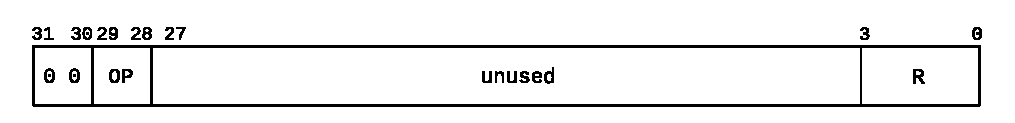
\includegraphics[width=\linewidth]{pictures/control_type_1.eps}
  \end{figure}  
  
  \hspace{-36px}\textbf{Type II}
  \begin{figure}[H]
    \centering
    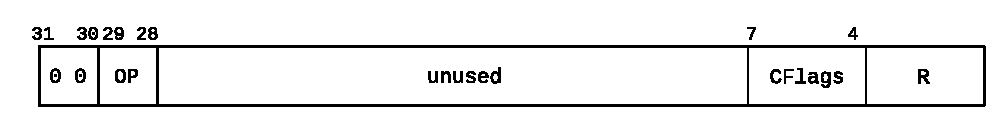
\includegraphics[width=\linewidth]{pictures/control_type_2.eps}
  \end{figure}  
  
  \hspace{-36px}\textbf{Type III}
  \begin{figure}[H]
    \centering
    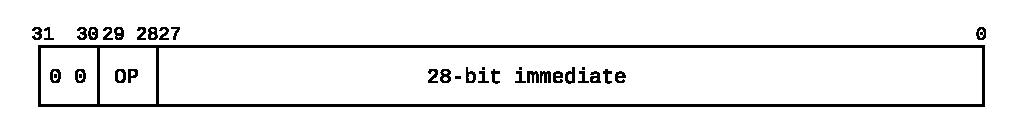
\includegraphics[width=\linewidth]{pictures/control_type_3.eps}
  \end{figure}  
  
  \FloatBarrier
  \begin{table}[H]
    \begin{center}
      \begin{tabular}[pos]{| c | l | l | l |} \hline 	
      \multicolumn{1}{|c|}{\cellcolor[gray]{0.9}\textbf{Type}} & 
      \multicolumn{1}{c|}{\cellcolor[gray]{0.9}\textbf{OP}} & 
      \multicolumn{1}{c|}{\cellcolor[gray]{0.9}\textbf{Opperation}} &
      \multicolumn{1}{c|}{\cellcolor[gray]{0.9}\textbf{Mnemonic}} \\ \hline
	 I 	& 00 & Jump Register	& jr r \\ \hline
	 I 	& 01 & Subroutine call  & call r \\ \hline
	 II 	& 10 & Branch flags 	& brfl r, const\\ \hline
	 III 	& 11 & Jump PC 		& jpc destiny\\ \hline	 
      \end{tabular}
    \end{center}
  \end{table}   
  
  \subsection{Memory}
  \begin{figure}[H]
    \centering
    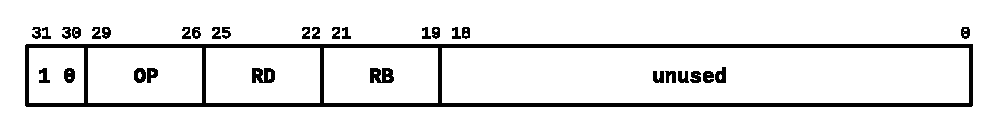
\includegraphics[width=\linewidth]{pictures/alu_instruction.eps}
  \end{figure} 
  
  \FloatBarrier
  \begin{table}[H]
    \begin{center}
      \begin{tabular}[pos]{| c | l | l |} \hline 	
      \multicolumn{1}{|c|}{\cellcolor[gray]{0.9}\textbf{OP}} & 
      \multicolumn{1}{c|}{\cellcolor[gray]{0.9}\textbf{Opperation}} & 
      \multicolumn{1}{c|}{\cellcolor[gray]{0.9}\textbf{Mnemonic}} \\ \hline
	 1000 & $R_D = Mem[R_B]$ 	& load d, b 	 \\ \hline
	 1100 & $Mem[R_B] = R_D$ 	& store b, d 	\\ \hline
      \end{tabular}
    \end{center}
  \end{table}   
  
  \section{Architecture Description}
  \label{sec:architecture_description}

  \subsection{Instruction Fetch}
  \subsubsection{Block Diagram}
  \begin{figure}[H]
    \centering
    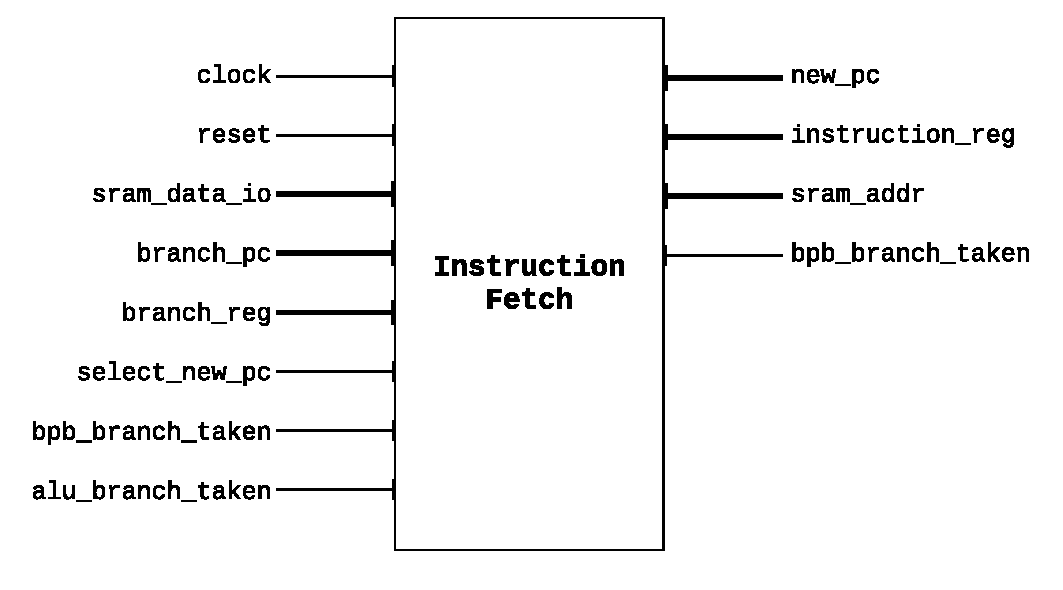
\includegraphics[width=\linewidth]{pictures/blocks/if_block.eps}
  \end{figure}    
  
  \subsubsection{Pin/Port Definitions}
  \FloatBarrier
  \begin{table}[H]
    \begin{center}
      \begin{tabular}[pos]{| l | c | c | m{7cm} |} \hline 	
      \multicolumn{1}{|c|}{\cellcolor[gray]{0.9}\textbf{Name}} & 
      \multicolumn{1}{c|}{\cellcolor[gray]{0.9}\textbf{Length}} & 
      \multicolumn{1}{c|}{\cellcolor[gray]{0.9}\textbf{Direction}} &
      \multicolumn{1}{c|}{\cellcolor[gray]{0.9}\textbf{Description}} \\ \hline
	 clock 		          & 1 	& input 	& CPU core clock  	\\ \hline
	 reset 		          & 1	  & input		& CPU core reset  	\\ \hline
	 sram\_data\_io     & 16	& in/out 	& SRAM data \\ \hline
	 branch\_pc 	      & 20	& input 	& Branch address PC relative \\ \hline
	 branch\_reg 	      & 20	& input 	& Branch address loaded from registers \\ \hline
   select\_new\_pc    & 1   & input   & Signal used for branch not taken \\ \hline
   bpb\_branch\_taken & 1   & input   & Branch prediction buffer result \\ \hline
   alu\_branch\_taken & 1   & input   & Branch result from execution \\ \hline
	 new\_pc 		        & 20	& output 	& Updated value of PC \\ \hline
	 instruction 	      & 32	& output 	& CPU core instruction  \\ \hline
	 sram\_addr 	      & 20	& output	& SRAM address \\ \hline
	 sram\_we 	        & 1	  & output 	& SRAM write enable  \\ \hline
   bpb\_branch\_taken & 1   & output  & Branch prediction buffer result \\ \hline
      \end{tabular}
    \end{center}
  \end{table} 

  \subsubsection{Internal Datapath} 
  The internal data path is composed by the following components.

  \begin{description}
    \item [Program Counter]: During the instruction time of an instruction this is the
address of the instruction word. The address of the instruction that occurs during
the next instruction time is determined by assigning a value to PC during an instruction time. If no value is assigned to PC during an instruction time by any pseudocode statement, it is automatically incremented by 2 before the next
instruction time.

  \end{description}

  \begin{figure}[H]
    \centering
    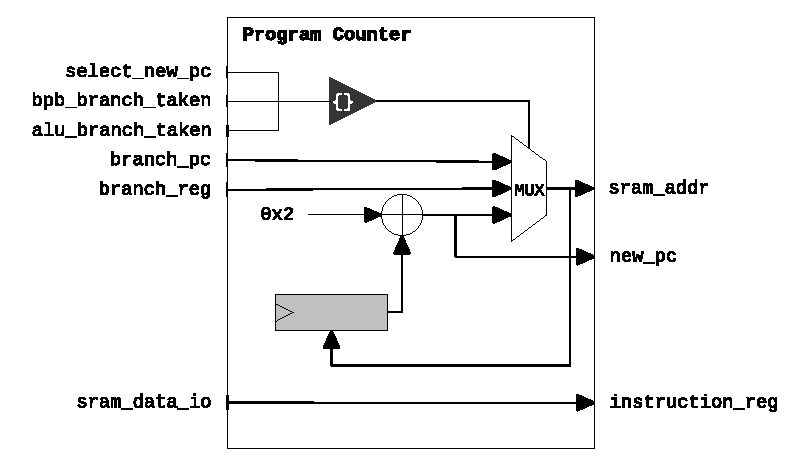
\includegraphics[width=\linewidth]{pictures/datapath/if_datapath.eps}
  \end{figure}   

  \newpage
  \subsection{Instruction Decode/Register Fetch}
  \subsubsection{Block Diagram}
  \begin{figure}[H]
    \centering
    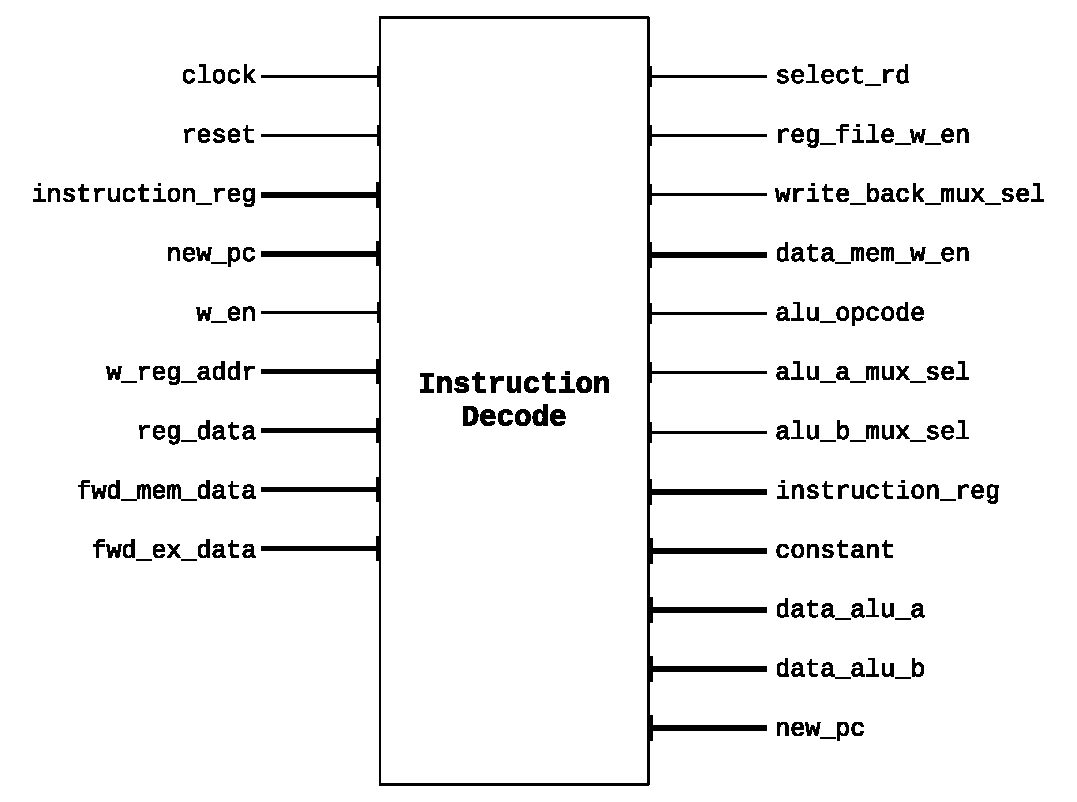
\includegraphics[width=\linewidth]{pictures/blocks/id_block.eps}
  \end{figure} 
  
  \subsubsection{Pin/Port Definitions}
  \FloatBarrier
    \begin{center}
      \begin{longtable}[pos]{| l | c | c | m{7cm} |} \hline       	
        \multicolumn{1}{|c|}{\cellcolor[gray]{0.9}\textbf{Name}} & 
        \multicolumn{1}{c|}{\cellcolor[gray]{0.9}\textbf{Length}} & 
        \multicolumn{1}{c|}{\cellcolor[gray]{0.9}\textbf{Direction}} &
        \multicolumn{1}{c|}{\cellcolor[gray]{0.9}\textbf{Description}} \\ \hline
        \endfirsthead
        \hline
        \multicolumn{4}{|l|}%
        {{\bfseries continued from previous page}} \\
        \hline
        \multicolumn{1}{|c|}{\cellcolor[gray]{0.9}\textbf{Name}} & 
        \multicolumn{1}{c|}{\cellcolor[gray]{0.9}\textbf{Length}} & 
        \multicolumn{1}{c|}{\cellcolor[gray]{0.9}\textbf{Direction}} &
        \multicolumn{1}{c|}{\cellcolor[gray]{0.9}\textbf{Description}} \\ \hline
        \endhead

        \hline \multicolumn{4}{|r|}{{continued on next page}} \\ \hline
        \endfoot

        \hline
        \endlastfoot

      	clock 		          & 1 	& input 	& CPU core clock  	\\ \hline
      	reset 		          & 1	  & input		& CPU core reset  	\\ \hline
      	instruction\_reg    & 32	& input 	& CPU core instruction \\ \hline
      	new\_pc 	          & 20	& input 	& Updated value of PC \\ \hline
      	w\_en 	            & 1	  & input 	& GPR bank write enable signal \\ \hline
      	w\_reg\_addr 	      & 4	  & input 	& GPR bank destiny address  \\ \hline
      	reg\_data 	        & 32	& input 	& GPR bank write data  \\ \hline
      	fwd\_mem\_data 	    & 32	& input	  & Forwarding data from DRAM output \\ \hline
      	fwd\_ex\_data 	    & 32	& input 	& Forwarding data from ALU output  \\ \hline
      	bpb\_branch\_taken  & 1   & input   & Branch prediction buffer result \\ \hline
        select\_rd 	        & TBD & output 	& TBD  \\ \hline
        reg\_file\_w\_en    & 1   & output  & GPR bank write enable \\ \hline
        write\_back\_mux\_sel & TBD & output & Write back mux select \\ \hline
        data\_mem\_w\_en    & 1  & output  & SDRAM write enable  \\ \hline
        alu\_opcode         & 3  & output  & ALU opperation code  \\ \hline
        select\_mux\_alu\_a & TBD& output  & ALU input A data select  \\ \hline
        select\_mux\_alu\_b & TBD& output  & ALU input B data select \\ \hline
        instruction\_reg    & 32 & output  & CPU core instruction  \\ \hline
        constant            & 32 & output  & 32-bit Sign-extended constant  \\ \hline
        data\_alu\_a        & 32 & output  & ALU input A data  \\ \hline
        data\_alu\_b        & 32 & output  & ALU input B data  \\ \hline
        new\_pc             & 20 & output  & Updated value of PC  \\ \hline
        bpb\_branch\_taken  & 1   & output   & Branch prediction buffer result \\ \hline

      \end{longtable}
    \end{center}

  \newpage
  \subsection{Execute/Address Calculate}
  \subsubsection{Block Diagram}
  \begin{figure}[H]
    \centering
    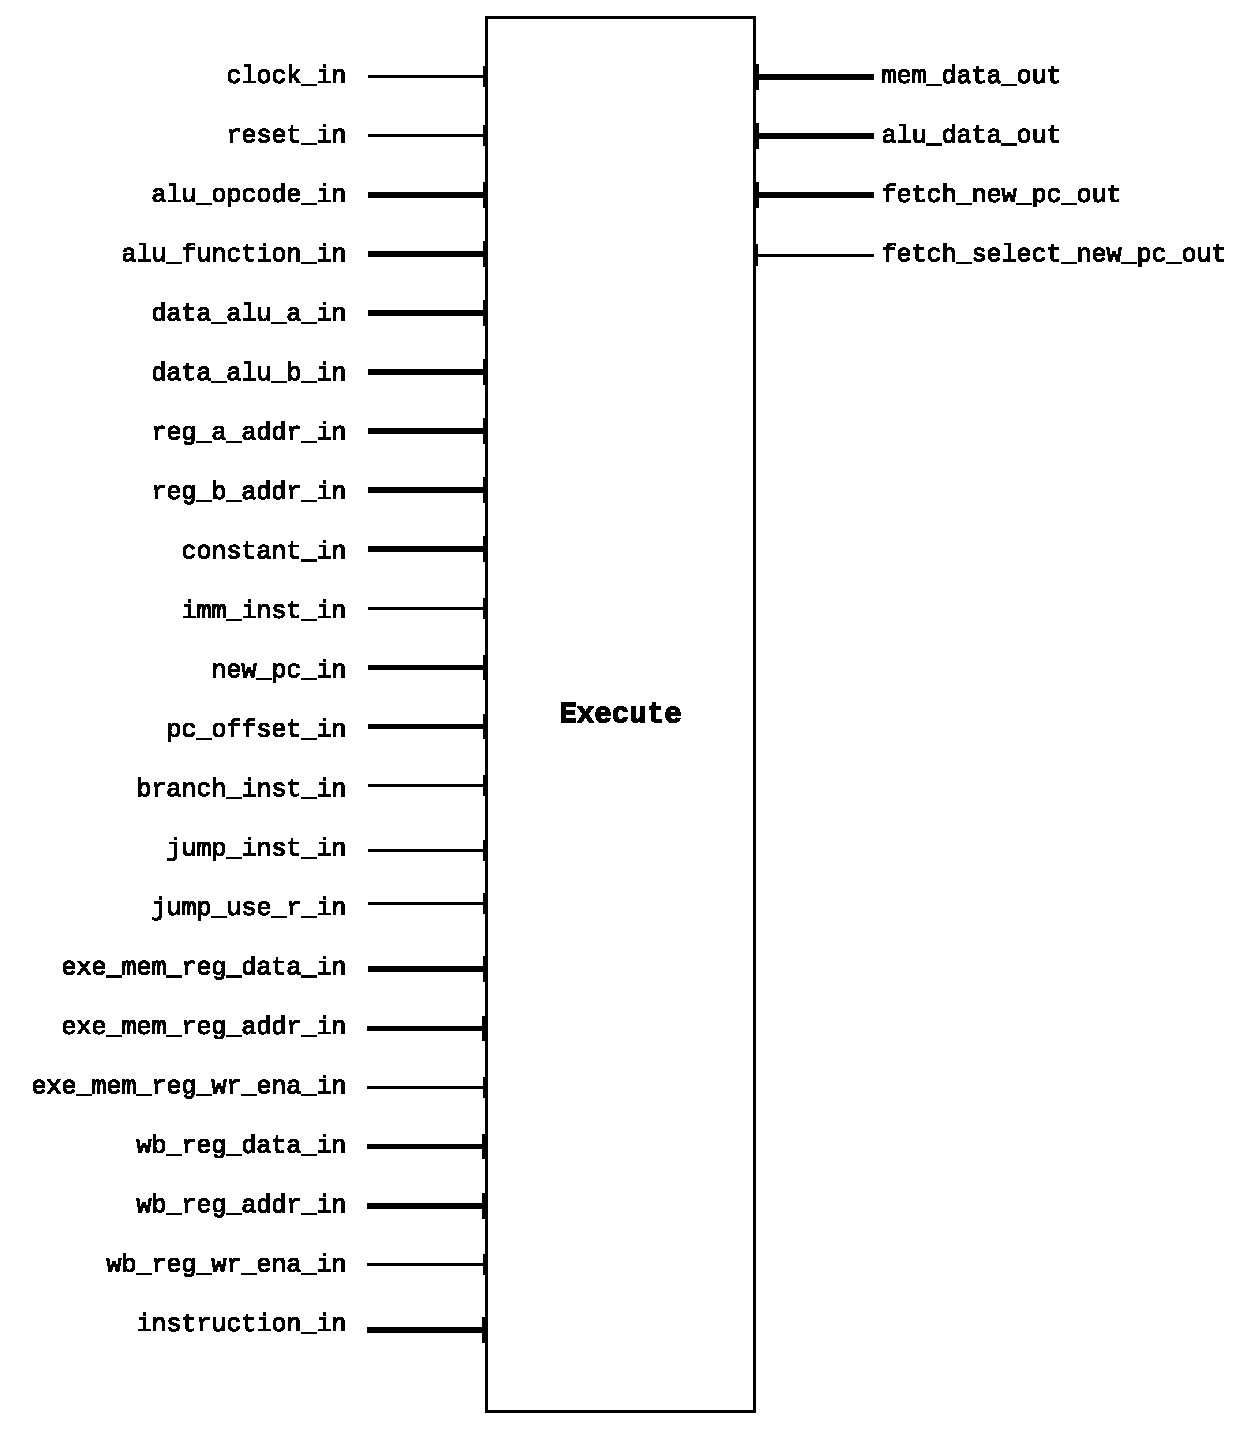
\includegraphics[width=\linewidth]{pictures/blocks/ex_block.eps}
  \end{figure} 

  \subsubsection{Pin/Port Definitions}
  \FloatBarrier
    \begin{center}
      \begin{longtable}[pos]{| l | c | c | m{7cm} |} \hline         
        \multicolumn{1}{|c|}{\cellcolor[gray]{0.9}\textbf{Name}} & 
        \multicolumn{1}{c|}{\cellcolor[gray]{0.9}\textbf{Length}} & 
        \multicolumn{1}{c|}{\cellcolor[gray]{0.9}\textbf{Direction}} &
        \multicolumn{1}{c|}{\cellcolor[gray]{0.9}\textbf{Description}} \\ \hline
        \endfirsthead
        \hline
        \multicolumn{4}{|l|}%
        {{\bfseries continued from previous page}} \\
        \hline
        \multicolumn{1}{|c|}{\cellcolor[gray]{0.9}\textbf{Name}} & 
        \multicolumn{1}{c|}{\cellcolor[gray]{0.9}\textbf{Length}} & 
        \multicolumn{1}{c|}{\cellcolor[gray]{0.9}\textbf{Direction}} &
        \multicolumn{1}{c|}{\cellcolor[gray]{0.9}\textbf{Description}} \\ \hline
        \endhead

        \hline \multicolumn{4}{|r|}{{continued on next page}} \\ \hline
        \endfoot

        \hline
        \endlastfoot

        clock               & 1   & input   & CPU core clock    \\ \hline
        reset               & 1   & input   & CPU core reset    \\ \hline
        alu\_opcode         & 3  & input  & ALU opperation code  \\ \hline
        data\_alu\_a        & 32 & input  & ALU input A data  \\ \hline
        data\_alu\_b        & 32 & input  & ALU input B data  \\ \hline
        alu\_a\_mux\_sel & TBD& input  & ALU input A data select  \\ \hline
        alu\_b\_mux\_sel & TBD& input  & ALU input B data select \\ \hline
        instruction\_reg    & 32 & input  & CPU core instruction  \\ \hline        
        constant            & 32 & input  & 32-bit Sign-extended constant  \\ \hline
        write\_back\_mux\_sel & TBD & input & Write back mux select \\ \hline  
        reg\_file\_w\_en    & 1   & input  & GPR bank write enable \\ \hline 
        select\_rd          & TBD & input  & TBD  \\ \hline
        bpb\_branch\_taken  & 1   & input   & Branch prediction buffer result \\ \hline
        new\_pc             & 20 & input  & Updated value of PC  \\ \hline    
        data\_alu\_a        & 32 & output  & ALU input A data  \\ \hline         
        alu\_data           & 32  & output  & ALU data output \\ \hline
        instruction\_reg    & 32 & output  & CPU core instruction  \\ \hline  
        write\_back\_mux\_sel & TBD & output & Write back mux select \\ \hline  
        reg\_file\_w\_en    & 1   & output  & GPR bank write enable \\ \hline 
        select\_rd          & TBD & output  & TBD  \\ \hline 
        branch\_result      & 1   & output  & Branch result after flag over ALU execution check

      \end{longtable}
    \end{center}  

  \newpage
  \subsection{Memory Access}
  \subsubsection{Block Diagram}
  \begin{figure}[H]
    \centering
    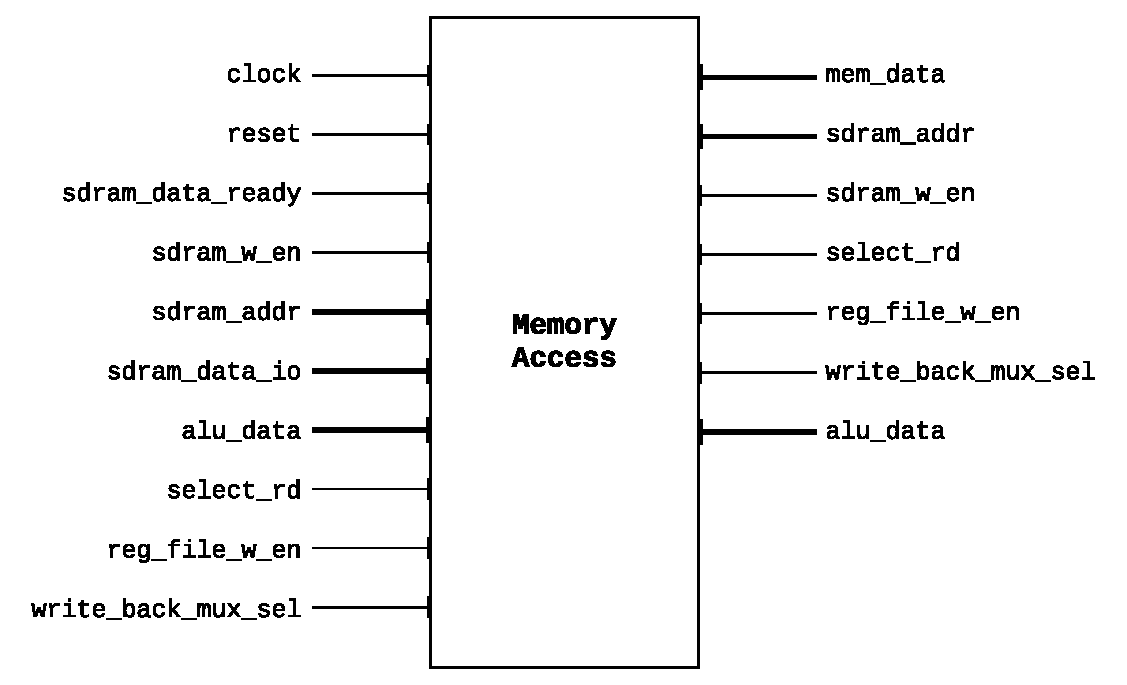
\includegraphics[width=\linewidth]{pictures/blocks/mem_block.eps}
  \end{figure} 

  \subsubsection{Pin/Port Definitions}
  \FloatBarrier
    \begin{center}
      \begin{longtable}[pos]{| l | c | c | m{7cm} |} \hline         
        \multicolumn{1}{|c|}{\cellcolor[gray]{0.9}\textbf{Name}} & 
        \multicolumn{1}{c|}{\cellcolor[gray]{0.9}\textbf{Length}} & 
        \multicolumn{1}{c|}{\cellcolor[gray]{0.9}\textbf{Direction}} &
        \multicolumn{1}{c|}{\cellcolor[gray]{0.9}\textbf{Description}} \\ \hline
        \endfirsthead
        \hline
        \multicolumn{4}{|l|}%
        {{\bfseries continued from previous page}} \\
        \hline
        \multicolumn{1}{|c|}{\cellcolor[gray]{0.9}\textbf{Name}} & 
        \multicolumn{1}{c|}{\cellcolor[gray]{0.9}\textbf{Length}} & 
        \multicolumn{1}{c|}{\cellcolor[gray]{0.9}\textbf{Direction}} &
        \multicolumn{1}{c|}{\cellcolor[gray]{0.9}\textbf{Description}} \\ \hline
        \endhead

        \hline \multicolumn{4}{|r|}{{continued on next page}} \\ \hline
        \endfoot

        \hline
        \endlastfoot

        clock               & 1   & input  & CPU core clock    \\ \hline
        reset               & 1   & input  & CPU core reset    \\ \hline
        sdram\_dara\_ready  & 1   & input  & SDRAM data ready control \\ \hline        
        sdram\_w\_en        & 1   & input  & SDRAM write enable \\ \hline        
        sdram\_addr         & 13  & input  & SDRAM read/write address \\ \hline
        sdram\_data\_io     & 32  & input  & SDRAM I/O data \\ \hline
        alu\_data           & 32  & input  & ALU data output \\ \hline  
        select\_rd          & TBD & input  & Select data to be writen in GPR bank \\ \hline                     
        reg\_file\_w\_en      & 4   & input  & GPR bank write enable signal \\ \hline
        write\_back\_mux\_sel  & TBD & input  & Write back mux select  \\ \hline

        mem\_data           & 32  & output & Memory output data  \\ \hline
        sdram\_addr         & 13  & output & SDRAM read/write address  \\ \hline
        sdram\_w\_en        & 1   & output & SDRAM write enable  \\ \hline
        select\_rd          & TBD & output & Select data to be writen in GPR bank \\ \hline                     
        reg\_file\_w\_en      & 4   & output  & GPR bank write enable signal \\ \hline
        write\_back\_mux\_sel  & TBD & output  & Write back mux select  \\ \hline

        alu\_data           & 32  & output & ALU data output \\ \hline 
      \end{longtable}
    \end{center}  
  
  \newpage
  \subsection{Write Back}
  \subsubsection{Block Diagram}
  \begin{figure}[H]
    \centering
    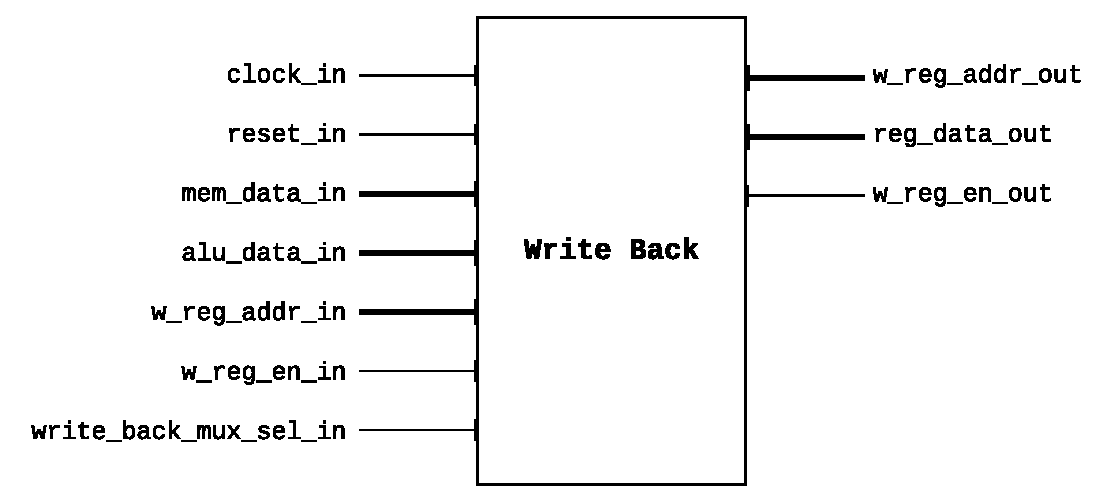
\includegraphics[width=\linewidth]{pictures/blocks/wb_block.eps}
  \end{figure} 

  \subsubsection{Pin/Port Definitions}
  \FloatBarrier
    \begin{center}
      \begin{longtable}[pos]{| l | c | c | m{7cm} |} \hline         
        \multicolumn{1}{|c|}{\cellcolor[gray]{0.9}\textbf{Name}} & 
        \multicolumn{1}{c|}{\cellcolor[gray]{0.9}\textbf{Length}} & 
        \multicolumn{1}{c|}{\cellcolor[gray]{0.9}\textbf{Direction}} &
        \multicolumn{1}{c|}{\cellcolor[gray]{0.9}\textbf{Description}} \\ \hline
        \endfirsthead
        \hline
        \multicolumn{4}{|l|}%
        {{\bfseries continued from previous page}} \\
        \hline
        \multicolumn{1}{|c|}{\cellcolor[gray]{0.9}\textbf{Name}} & 
        \multicolumn{1}{c|}{\cellcolor[gray]{0.9}\textbf{Length}} & 
        \multicolumn{1}{c|}{\cellcolor[gray]{0.9}\textbf{Direction}} &
        \multicolumn{1}{c|}{\cellcolor[gray]{0.9}\textbf{Description}} \\ \hline
        \endhead

        \hline \multicolumn{4}{|r|}{{continued on next page}} \\ \hline
        \endfoot

        \hline
        \endlastfoot

        clock               & 1   & input  & CPU core clock    \\ \hline
        reset               & 1   & input  & CPU core reset    \\ \hline
        mem\_data           & 32  & input  & SDRAM data output \\ \hline
        alu\_data           & 32  & input  & ALU data output \\ \hline
        w\_file\_w\_en      & 4   & input  & GPR bank write enable signal \\ \hline
        w\_reg\_addr        & 1   & input  & GPR bank destiny address  \\ \hline
        write\_back\_mux\_sel  & TBD & input  & Write back mux select  \\ \hline
        select\_rd          & TBD & input  & Select data to be writen in GPR bank \\ \hline
        w\_reg\_addr        & 4   & output & GPR bank destiny address  \\ \hline
        reg\_data           & 32  & output & GPR bank write data  \\ \hline
        reg\_file\_w\_en    & 1  & output  & GPR bank write enable signal  \\ \hline
      \end{longtable}
    \end{center}  

  \subsubsection{Internal Datapath} 
  The internal data path is composed by the following components.

  \begin{figure}[H]
    \centering
    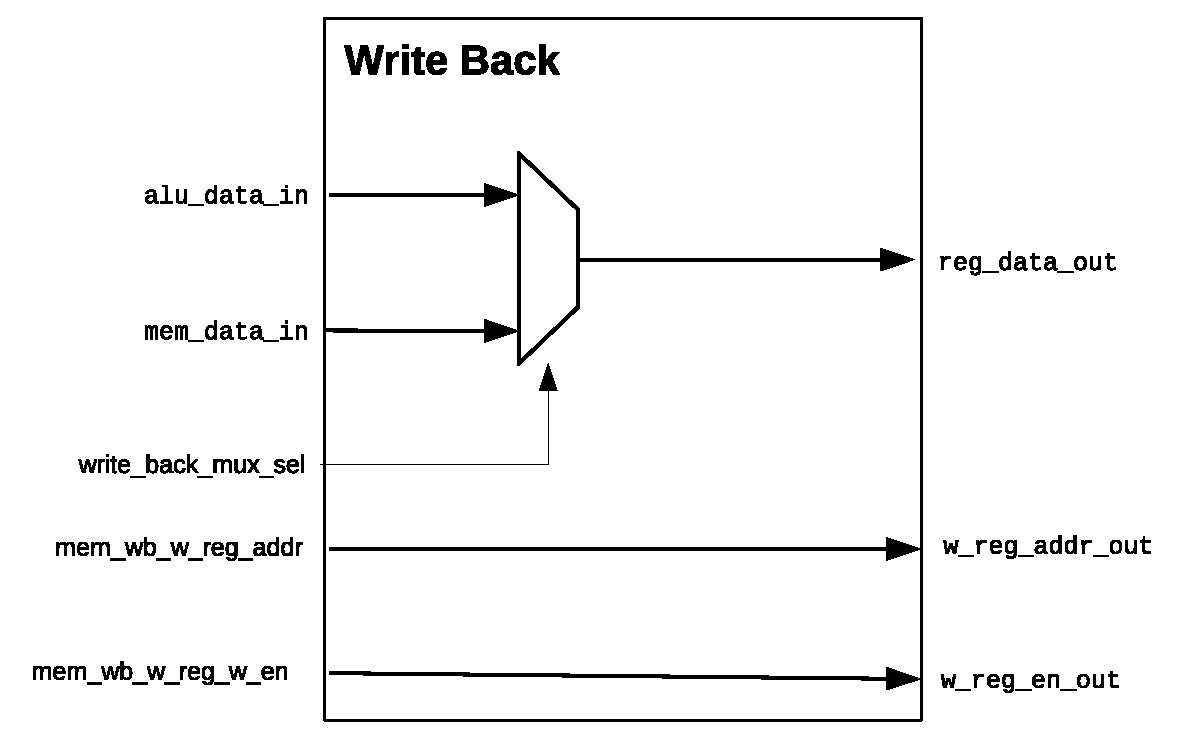
\includegraphics[width=\linewidth]{pictures/datapath/wb_datapath.eps}
  \end{figure}      
  
  \newpage
  \subsection{Pipeline Register Description}
  \subsubsection{Instruction Fetch/Instruction Decode}

  \FloatBarrier
    \begin{center}
      \begin{longtable}[pos]{| l | c | m{9cm} |} \hline         
        \multicolumn{1}{|c|}{\cellcolor[gray]{0.9}\textbf{Name}} & 
        \multicolumn{1}{c|}{\cellcolor[gray]{0.9}\textbf{Length}} & 
        \multicolumn{1}{c|}{\cellcolor[gray]{0.9}\textbf{Description}} \\ \hline
        \endfirsthead
        \hline
        \multicolumn{3}{|l|}%
        {{\bfseries continued from previous page}} \\
        \hline
        \multicolumn{1}{|c|}{\cellcolor[gray]{0.9}\textbf{Name}} & 
        \multicolumn{1}{c|}{\cellcolor[gray]{0.9}\textbf{Length}} & 
        \multicolumn{1}{c|}{\cellcolor[gray]{0.9}\textbf{Description}} \\ \hline
        \endhead

        \hline \multicolumn{3}{|r|}{{continued on next page}} \\ \hline
        \endfoot

        \hline
        \endlastfoot

        new\_pc           & 20  & Stores the next program counter value.\\ \hline
        instruction\_reg  & 32  & Stores the intruction word.    \\ \hline
        bpb\_branch\_taken       & 1   & Stores BPB result. \\ \hline

      \end{longtable}
    \end{center} 

  \subsubsection{Instruction Decode/Execute}

  \FloatBarrier
    \begin{center}
      \begin{longtable}[pos]{| l | c | m{9cm} |} \hline         
        \multicolumn{1}{|c|}{\cellcolor[gray]{0.9}\textbf{Name}} & 
        \multicolumn{1}{c|}{\cellcolor[gray]{0.9}\textbf{Length}} & 
        \multicolumn{1}{c|}{\cellcolor[gray]{0.9}\textbf{Description}} \\ \hline
        \endfirsthead
        \hline
        \multicolumn{3}{|l|}%
        {{\bfseries continued from previous page}} \\
        \hline
        \multicolumn{1}{|c|}{\cellcolor[gray]{0.9}\textbf{Name}} & 
        \multicolumn{1}{c|}{\cellcolor[gray]{0.9}\textbf{Length}} & 
        \multicolumn{1}{c|}{\cellcolor[gray]{0.9}\textbf{Description}} \\ \hline
        \endhead

        \hline \multicolumn{3}{|r|}{{continued on next page}} \\ \hline
        \endfoot

        \hline
        \endlastfoot

        new\_pc                 & 20  & Stores the next program counter value.\\ \hline
        data\_alu\_reg\_a       & 32  & Stores the value of ALU input port A.  \\ \hline
        data\_alu\_reg\_b       & 32  & Stores the value of ALU input port B. \\ \hline
        constant                & 32  & Stores the signed extended integer constant. \\ \hline
        instruction\_reg        & 32  & Stores the intruction word.    \\ \hline
        select\_rd\_reg           & 1   & TBD  \\ \hline
        reg\_file\_w\_en\_reg       & 1   & Stores the signal to enable GPR write back. \\ \hline
        write\_back\_mux\_sel\_reg  & TBD & Stores the select signal for write back Multiplexer. \\ \hline
        alu\_opcode              & 3   & Stores the ALU opperation code. \\ \hline
        select\_mux\_alu\_a        & TBD & Stores the ALU input data select signal \\ \hline
        select\_mux\_alu\_b        & TBD & Stores the ALU input data select signal \\ \hline
        bpb\_branch\_taken       & 1   & Stores BPB result. \\ \hline

      \end{longtable}
    \end{center} 

\subsubsection{Execute/Memory Access}

  \FloatBarrier
    \begin{center}
      \begin{longtable}[pos]{| l | c | m{9cm} |} \hline         
        \multicolumn{1}{|c|}{\cellcolor[gray]{0.9}\textbf{Name}} & 
        \multicolumn{1}{c|}{\cellcolor[gray]{0.9}\textbf{Length}} & 
        \multicolumn{1}{c|}{\cellcolor[gray]{0.9}\textbf{Description}} \\ \hline
        \endfirsthead
        \hline
        \multicolumn{3}{|l|}%
        {{\bfseries continued from previous page}} \\
        \hline
        \multicolumn{1}{|c|}{\cellcolor[gray]{0.9}\textbf{Name}} & 
        \multicolumn{1}{c|}{\cellcolor[gray]{0.9}\textbf{Length}} & 
        \multicolumn{1}{c|}{\cellcolor[gray]{0.9}\textbf{Description}} \\ \hline
        \endhead

        \hline \multicolumn{3}{|r|}{{continued on next page}} \\ \hline
        \endfoot

        \hline
        \endlastfoot

        instruction\_reg        & 32  & Stores the intruction word.    \\ \hline
        select\_rd\_reg         & 1   & TBD  \\ \hline
        reg\_file\_w\_en\_reg   & 1   & Stores the signal to enable GPR write back. \\ \hline
        write\_back\_mux\_sel\_reg  & TBD & Stores the select signal for write back Multiplexer. \\ \hline
        data\_alu\_a            & 32  & Stores the ALU input data A for memory addressing. \\ \hline
        alu\_data\_reg          & 32  & Stores the ALU output data. \\ \hline
      \end{longtable}
    \end{center}  

\subsubsection{Memory Access/Write Back}

  \FloatBarrier
    \begin{center}
      \begin{longtable}[pos]{| l | c | m{9cm} |} \hline         
        \multicolumn{1}{|c|}{\cellcolor[gray]{0.9}\textbf{Name}} & 
        \multicolumn{1}{c|}{\cellcolor[gray]{0.9}\textbf{Length}} & 
        \multicolumn{1}{c|}{\cellcolor[gray]{0.9}\textbf{Description}} \\ \hline
        \endfirsthead
        \hline
        \multicolumn{3}{|l|}%
        {{\bfseries continued from previous page}} \\
        \hline
        \multicolumn{1}{|c|}{\cellcolor[gray]{0.9}\textbf{Name}} & 
        \multicolumn{1}{c|}{\cellcolor[gray]{0.9}\textbf{Length}} & 
        \multicolumn{1}{c|}{\cellcolor[gray]{0.9}\textbf{Description}} \\ \hline
        \endhead

        \hline \multicolumn{3}{|r|}{{continued on next page}} \\ \hline
        \endfoot

        \hline
        \endlastfoot

        instruction\_reg        & 32  & Stores the intruction word.    \\ \hline
        select\_rd\_reg         & 1   & TBD  \\ \hline
        reg\_file\_w\_en\_reg   & 1   & Stores the signal to enable GPR write back. \\ \hline
        write\_back\_mux\_sel\_reg  & TBD & Stores the select signal for write back Multiplexer. \\ \hline
        mem\_data\_reg          & 32  & Stores the memory output data. \\ \hline
        alu\_data\_reg          & 32  & Stores the ALU output data. \\ \hline
        w\_reg\_addr\_reg       & 4   & Stores the GPR data write address. \\ \hline

      \end{longtable}
    \end{center}   

  \subsection{SRAM Controller}
  TBD in further releases?

  \subsection{SDRAM Controller}
  TBD in further releases?

  \subsection{Forwarding Unit}
  TBD in further releases.

  \subsection{Branch Prediction Buffer}
  TBD in further releases.
  
  \subsection{Control Micro-instructions Description}
 
  \subsection{Bootloader}
  TBD in further releases.

  %\newpage
  %\section{Timing}
    
% \bibliographystyle{ieeetr}
% \bibliography{ipprocess}

\end{document}
